In diesem Kapitel werden die Arbeitsprozesse der Evaluation und Optimierung reflektiert. Des Weiteren geht es darum, Vorschläge zu unterbreiten, die den Prozess unterstützen, dass optimale Sprachmodell auszuwählen.\vspace{0.2cm}

Zudem werden die größten Hindernisse und Probleme besprochen, die während des gesamten Prozesses der Evaluation auftraten. Diese beinhalten die Bereitstellung er Modelle, das Erheben der Daten von den Proben des Benchmarks und deren Auswertung. Um in folgenden Arbeiten diese Fehler zu verhindern werden dazu Lösungsansätze und Vorschläge diskutiert.

% --- Evaluierung ----------------------------------------------------------------------------------


\section{Evaluierungsaufbau und Vorbereitung}
Um die Evaluierungen an Open-Source-Modellen durchführen zu können, mussten diese lokal bereitgestellt werden. Die Wahl viel auf das Ollama-Framework, da die Installation und Konfiguration sehr gut durch die Entwicklungsfirma und verschiedene Foren unterstützt wird. Neben der vorhandenen API lässt sich das Tool \textit{Open-WebUI} einfach in das Ollama-Frameowrk integrieren. Dieses Tool bietet eine gute UI die von allen Clients mit dem Browser im Netzwerk aufgerufen werden kann. Ebenfalls ein großer Vorteil sind die vielen Modelle welche für Ollama zum Download bereitstehen. Darunter sind Modelle von KI-Entwicklungsfirmen, wie Mistral, Llama, Deepseek und Qwen-Coder.\vspace{0.2cm}

Eine weitere Möglichkeit ist, die Modelle lokal auszuführen ohne ein Framework einzusetzen. Hierbei können die Abfragen nur auf dem lokalen System erfolgen, wenn keine eigene API Schnittstelle erstellt wird. Des Weiteren fehlte auch eine Web-UI Lösung, sodass diese Möglichkeit nicht weiter in Betracht gezogen wurde.\vspace{0.2cm}

Für die Evaluierung der kommerziellen Closed-Source-Modelle ist dieser Schritt nicht erforderlich. Hier wird lediglich ein Zugang, in Form eines API-Schlüssels benötigt.\vspace{0.2cm}

%---------------------------------------------------------------------------------------------------


\section{Evaluierung der großen Sprachmodelle}
Ein großes Problem stellte der Zugriff auf die Cloused-Source-Modelle dar. Durch die beschränkten Bezahlmethoden konnte ein permanenter Zugriff auf die Modelle nicht erfolgen. Aus diesem Grund wurden hauptsächlich Open-Source-Modelle lokal evaluiert und getestet. Bei der Optimierung sind ausschließlich Open-Source-Modelle zu Einsatz gekommen.


\subsection{Lokale Ressourcen}
Eines der größten Probleme für das lokale Betreiben von großen Sprachmodellen sind die Hardwareanforderungen. Hier spielen neben der Prozessoranzahl, der Speicherplatz auf der Festplatte, der RAM und der VRAM der Grafikkarte eine entscheidende Rolle. Während der Arbeit wurde eine SSD-Festplatte mit höherer Kapazität eingesetzt und die Grafikkarte, durch eine andere mit größeren VRAM ersetzt.\vspace{0.2cm}

Die größere SSD-Festplatte wurde notwendig, während des Ladens und Speichern der Modelle mithilfe des Ollama Framework. Speziell für das Speichern der Modelle, war ein RAM notwendig, der doppelt so groß sein musste, wie das Modell selbst. Um diesen RAM bereit zustellen wurde eine SWAP Partition von 100 GB auf der SSD eingerichtet. Dies stellte eine kosten günstigere Variante dar, als der Erwerb von echtem RAM. Dieser emulierte RAM wurde auch für die Ausführung größerer Modelle benötigt, bei der Verwendung von der Grafikkarte mit 4 GB VRAM.\vspace{0.2cm}

Eine weitere und signifikante Verbesserung brachte der Austausch der Grafikkarte. Hierbei wurde die vorhandene Nvidia GTX 1050 TI mit 4 GB \acrshort{VRAM} und einer Bandbreite von 112 GB/s durch eine Nvidia RTX 3060 mit 12 GB VRAM und einer Bandbreite von 360 GB/s ersetzt. Durch den Austausch der Grafikkarte wurde die eingerichtete SWAP Partition nicht mehr benötigt und die RAM Auslastung ist auch bei den größeren Modellen stark gesunken.

Durch diese Anpassungen der Hardware bestand nun die Möglichkeit größere Modelle zuladen und bereit zustellen. Des Weiteren konnte eine wesentliche Verbesserung der Antwortzeit festgestellt werden. So wurde bei dem \textit{Deekseek-Coder-V2} Modell eine Verbesserung der Berechnungszeit für den Benchmark von etwa 24 Stunden auf circa eine Stunde beobachtet. Da der Fokus dieser Arbeit nicht auf eine Optimierung der Hardware liegt, wird auf eine genaue Messung der Antwortzeiten verzichtet.\vspace{0.2cm}

Dennoch war die Berechnungszeit für die Generierung der Codes bei einigen Modellen, die mehr als 12 GB groß waren sehr hoch. Sodass die Wartezeit, das Auswerten der Evaluierung verzögerte.


\subsection{Auswertung des Benchmarks}
Die Anwendung des vorgeschlagenen Parametersatzes zeigte bemerkenswerte unerwünschte Auswirkungen auf die Erzeugung der Antworten. Insbesondere bei einer Tokenlänge von 600 traten Störungen auf, bei denen einige Modelle unbrauchbaren Code generierten. Dieser Umstand, resultierte beim \textit{DeepSeek-R1} aus einem '<think>'-Abschnitt innerhalb der Antwortstruktur, in dem das Modell eine detaillierte Herleitung seines Denkprozesses anbietet, bevor es zur eigentlichen Lösung gelangte. Bei dem Modell \textit{Gemini 1.5} führten ausführliche Erklärungen am Anfang und Ende der Antwort zum selben Effekt, sodass diese Ergebnisse ebenfalls nicht brauchbar waren. Aus diesem Grund wurde bei den Modellen \textit{DeepSeek-R1} und \textit{Gemini 1.5} auf eine Einschränkung der Tokenlänge verzichtet.\vspace{0.2cm}

Die hohen Erwartungen bei den Resultaten der kommerziellen Closed-Source-Modelle wurden nicht erfüllt. Die Modelle, \textit{Gemini 1.5} mit einem \texttt{pass@1} Ergebnis von 29,25\% und \textit{ChatGPT} 4 mit 33,5\% liegen somit im unteren Bereich der Auswertung und werden von vielen Open-Source-Modellen übertroffen. Auf eine erneute Evaluierung des OpenAI Modell musste aus Kostengründen verzichtet werden.
% Beispiel
Zu einem ähnlichen Ergebnis kommt die Fallstudie, welche in \cite{ahmed-2025} vorgestellt wird. Bewertet wurde hier der generierte Code von ChatGPT 4 und dessen Nutzen für die Gestaltung einer barrierefreien Webseite. Die Studie kommt zu dem Schluss, dass ChatGPT für den Entwickler ein nützliches Tool darstellt, aber das Urteilsvermögen und Fachwissen des Entwicklers nicht ersetzen kann \parencite[vgl.][10]{ahmed-2025}.\vspace{0.2cm}

Bei der Auswertung des Benchmarks traten einige Fehler auf, die weitestgehend beseitigt werden konnten. Ein Großteil waren kleinere Fehler, die bei der Auswertung aufgetreten, die in Kapitel \ref{subsec:disadvantages_of_evaluation} noch ausführlicher besprochen werden. Der gravierendste Fehler trat aber bei der Berechnung das \texttt{pass@k} für das gesamte Modell auf. Hier wurde eine falsche Python-Methode implementiert, sodass die Ergebnisse, um ein Vielfaches niedriger waren. Erst durch den Vergleich mit Ergebnisse anderer Arbeiten und den Herstellerangaben ist der Fehler aufgefallen. Nach intensiver Suche wurde dieser schlussendlich gefunden und beseitigt.\vspace{0.2cm}

Bewehrt hat sich der Einsatz von Python und dessen Bibliotheken für Umsetzung der Evaluierungs- und Optimierungsaufgaben. Mittlerweile existieren für die meisten Probleme und Anforderungen, fertige Bibliotheken. Oft von den Herstellern der Modelle selbst. Basierend auf den vorhandenen Bibliotheken, konnte die Entwicklung der Evaluationsaufgaben in kurzer Zeit umgesetzt und implementiert werden.\vspace{0.2cm}

% --- Evalierung mit eigenen ---------------------------------


\subsection{Nachteile der Evaluierung}\label{subsec:disadvantages_of_evaluation}
Trotz seines häufigen Einsatzes bei der Evaluierung von Modellen, in verschiedenen wissenschaftlichen Arbeiten, zeigt der Benchmark-Test für die deutschen PHP Proben Fehler. Aber auch bei der Erstellung der Auswertung mit Python traten Fehler auf. Dadurch entstehen Nachteile für die Modelle, bei der Bewertung mit dem HumanEval-XL Benchmark. Im Verlauf dieses Kapitels werden einige Nachteile diskutiert.\vspace{0.2cm}

Bei der Probe \textit{php/5} wurde eine \textit{\textbf{nicht eindeutige Übersetzung}} festgestellt. So wurde die Probe übersetzt, nicht aber die Tests. Das Listing \ref{lst:prompt_php_de_5} zeigt die gültigen Werte welche als Eingabeparameter für die zu generierende Funktion erlaubt sind. Hier handelt es sich um deutsche Zahlworte von $null$ bis $neun$. Im angegebenen Beispieltest sind Eingabe- und Ausgabeparameter in englischer Sprache. Es wird auch nicht explizit angegeben, das eine Übersetzung erfolgen soll.\vspace{0.2cm}

\begin{lstlisting}[
language=php,
label=lst:prompt_php_de_5,
caption={Aufgabenstelleung der Probe php/5}
]
/**
 * Sie sind ein erfahrener PHP-Programmierer und hier ist Ihre Aufgabe.
 * Die Eingabe ist ein durch Leerzeichen getrennter String von Ziffern von 'null' bis 'neun'.
 *     Gültige Optionen sind 'null', 'eins', 'zwei', 'drei', 'vier', 'fünf', 'sechs', 'sieben', 'acht' und 'neun'.
 *     Gib den String mit den Zahlen sortiert von klein nach groß zurück.
 * >>> sort_numbers('three one five')
 * 'one three five'
 *
 */
function sortNumbers($numbers){
\end{lstlisting}

Die Probe \textit{php/5}, welcher in Listing \ref{lst:test_php_de_5} zu sehen ist, stellt einen Test zur Verfügung der die Prüfung mit englischem Zahlworten von $zero$ bis $nine$ ausführt. Keines der getesteten Modelle hat diese Probe bestanden. Alle getesteten Modelle haben Codes generiert, die deutsche Zahlwörter als Parameter erwarten um diese zu sortieren. Die englischen Zahlwörter werden durch die Methoden nicht als Zahlworte erkannt. Dadurch hat kein Modell diesen Test bestanden.\vspace{0.2cm}

\begin{lstlisting}[
	language=php,
	label=lst:test_php_de_5,
	caption={Aufgabenstelleung der Probe php/5}
]
// more tests.

$arg40 = "six five four three two one zero";
$x4 = sortNumbers($arg40);
$v4 = "zero one two three four five six";
if (!compare($x4, $v4)) {
    throw new Exception("Error at 5th assert statement.");
}
// more tests
\end{lstlisting}

Eine mögliche Lösung ist es, die Anpassung des Benchmarks vorzunehmen und alle Übersetzungen anzupassen oder zu korrigieren. Mit der originalen Benchmark in Deutsch und mit PHP, hat beispielsweise das Modell \textit{Deepseek Coder V2} keine korrekte Lösung generieren können. Wird der Test im Benchmark angepasst und die Zahlworte ebenfalls übersetzt, so wie der in Listing \ref{lst:test_php_de_5_translated} gezeigte Codeabschnitt, wird die Probe von dem Modell mit drei korrekten Antworten bestanden. Derselbe Test in der englischen Sprache wurde beispielsweise vom Modell \textit{Llama3.3} in allen fünf Antworten, mit bestanden bewertet. Da in der englischen Probe alle Zahlwörter in Englisch aufgeführt sind, ist anzunehmen das bei dieser Probe eine Übersetzung nicht das Ziel ist.\vspace{0.2cm}

\begin{figure}[!ht]
\begin{lstlisting}[
	language=php,
	label=lst:test_php_de_5_translated,
	caption={Übersetzte Aufgabenstelleung der Probe php/5}
]
// more tests.

$arg40 = "sechs fünf vier drei zwei eins null";
$x4 = sortNumbers($arg40);
$v4 = "null eins zwei drei vier fünf sechs";
if (!compare($x4, $v4)) {
    throw new Exception("Error at 5th assert statement.");
}
// more tests
\end{lstlisting}
\end{figure}

Die Ergebnisse vor und nach der Änderung für die fünfte Probe sind im Listing \ref{lst:test_php_de_5_translated_bash_view} für das Modell \textit{Deepseek Coder V2} dargestellt. Nach dem Namen $php/5$ wird die Gesamtanzahl der Proben angegeben, gefolgt von den insgesamt bestandenen Durchläufe der Probe. Anschließend werden die Wahrscheinlichkeiten, das eine korrekte Antwort unter den TOP Antworten zu finden ist, angegeben, beginnend mit dem \texttt{pass@1}.\vspace{0.2cm}

\begin{lstlisting}[
	language=bash,
	label=lst:test_php_de_5_translated_bash_view,
	caption={Ergebnisse der Probe php/5 für das \textit{Deepssek Coder V2} Modell}
]
# origin sample no. 5
php/5;5;0;0.0000;0.0000;0.0000;0.0000;0.0000

# translated sample no. 5
php/5;5;3;0.6000;0.9000;1.0000;1.0000;1.0000
\end{lstlisting}

Diese Probe zeigt, nach der Änderung wurden drei von fünf möglichen Antworten mit korrekt bewertet. Die Änderung für die Bewertung der \texttt{pass@k} Methode des gesamten Modells ist in Tabelle \ref{tab:pass_at_k_results_bevor_after_translate} dargestellt. Diese Änderung wurde nicht mehr auf alle Modelle ausgeweitet, sodass der Fehler in allen Bewertungen enthalten ist.\vspace{0.2cm}

\begin{table}[!ht]
	\begin{tabular}{|l|lllll|}
		\hline
		k & 1 & 2 & 3 & 4 & 5 \\
		\hline
		ohne Korrektur & 0,555 & 0,6112 & 0,6312 & 0,6425 & 0,65 \\
		mit Korrektor  & 0,565 & 0,6225 & 0,6438 & 0,6550 & 0,6625 \\
		\hline
		\hline
	\end{tabular}\centering
	\label{tab:pass_at_k_results_bevor_after_translate}
	\caption{Ergebnisse für das \textit{Deepseek Coder V2} Modell mit und ohne Probe 5 Korrektur }
\end{table}

Mit diesem Problem wird gezeigt, dass bereits ein kleiner Fehler das Ergebnis um mehr als ein Prozent für ein Modell verbessern kann.\vspace{0.2cm}

Eine andere Fehlerquelle ist das \textit{\textbf{Zusammenführen der Antworten der Modelle und den Tests aus dem Benchmark}}. Diese Fehlerquelle ist nicht der Benchmark selbst, sondern die Umsetzung der Ausführung und Bewertung. Oft sind die Probleme das Parsen der Sonderzeichen, wie beispielsweise die Verwendung der doppelten Anführungszeichen im Test und den erstellten Antworten. Eine manuelle Prüfung der Aufgabe 2 hat das Fehlverhalten aufgezeigt. Durch das Implementieren einiger weiteren Codezeilen in Python, wie das Listing \ref{lst:error_evaluation_code_1} zeigt, konnten die Bewertung einiger Modelle verbessert werden. So hat sich das Ergebnis für die \textit{pass@1} Methode des Deepseek-Coder-V2 um 7\% von $0,53$ auf $0,6$ verbessert. Ebenso wurde für das Llama3.1 Modell eine Verbesserung der Bewertung um $0,025$, von $0,45$ auf $0,475$ ermittelt.\vspace{0.2cm}

\begin{lstlisting}[
	language=diff,
	label=lst:error_evaluation_code_1,
	caption={Fehler bei der Auswertung durch fehlerhafte Anführungszeichen}
]
answer = answer.replace(r"\n", "\n")
+ answer = answer.replace(r'\"', '"')
+ 
+ test = test.replace(r'\"', '"') 
\end{lstlisting}

Ein weiteres Problem, welches sich in den Tests gezeigt hat, sind die von einigen Modellen \textit{\textbf{geänderten Methodennamen}}. Einige Modelle ändern diesen ab und passen ihn an die Funktionalität der Methode an. Dieses Verhalten ist beispielsweise beim Google Modell \textit{Gemini 1.5} mehrfach aufgetreten. Ein Beispiel ist die Probe 26 aus dem Benchmark. Hierbei sollte das $n$-te Element der Fibonacci-Folge berechnet werden. Der geforderte Name der Methode war als \texttt{fibfib} definiert. Das Modell schlug in einem Durchlauf den Namen \texttt{fibfib\_iterativ} vor, da über ein beliebig großes $n$ iteriert wird. Somit ist der Test für diese Probe fehlgeschlagen, obwohl die Methode die Berechnung korrekt durchführte. Dies wurde durch händische Änderungen am PHP Code überprüft und alle generierten Codes dieser Probe wurden bestanden. Das Listing \ref{lst:correct_func_with_non_correct_name} zeigt diese durch \textit{Gemini 1.5} generierte Funktion.\vspace{0.2cm}

\begin{lstlisting}[
	language=php,
	label=lst:correct_func_with_non_correct_name,
	caption={Generierte Funktion mit falschen Namen}
]
function fibfib_iterativ($n) {
    if ($n < 0) {
        throw new InvalidArgumentException("n muss nicht-negativ sein");
    }

    if ($n <= 2) {
        return $n - 1;
    }

    $a = 0;
    $b = 0;
    $c = 1;
    for ($i = 3; $i <= $n; $i++) {
        $temp = $a + $b + $c;
        $a = $b;
        $b = $c;
        $c = $temp;
    }
    return $c;
}
\end{lstlisting}

Ein Entwickler würde den Methodennamen anpassen und die Methode einsetzen. Eine Möglichkeit dies zu umgehen, ist es, den Methodennamen zur Laufzeit zu ermitteln. Mit den Proben sollen die Fähigkeiten der LLMs geprüft werden, inwieweit diese, grundlegende Funktionen implementieren können. Hierbei ist der Name der Methode nicht entscheidend. Anders würde es sich verhalten, wenn es sich dabei um Erweiterungen bestehender Programme handeln würde, in denen die erstellten Funktionen integriert werden soll.\vspace{0.2cm}

Die Tests aus dem Benchmark und Ergebnisse der Modelle wurde stichprobenartig manuell geprüft und weitere Fehler behoben. Dennoch ist nicht auszuschließen das die jetzige Evaluation weitere Fehlerquellen enthält.\vspace{0.2cm}

Es gibt durchaus weitere Fehlerquellen, welche die Ergebnisse negativ beeinflussen können. Beispielsweise könnten bei der Formulierung der Tests, Randbedingungen nicht korrekt betrachtet wurden und die Modelle die Aufgabe falsch interpretieren und so die Aufgabe falsch lösen. Oder Tests enthalten gänzlich falsche Parameter und richtig generierter Code wird trotzdem als Falsch gewertet. Die eben genannten Fehler oder ähnliche, konnten im vorliegenden Benchmark nicht nachgewiesen werden, ganz auszuschließen sind sie aber nicht.\vspace{0.2cm}

% --- Optimierung ----------------------------------------------------------------------------------


\section{Optimierung der Abfragen}
Die Tests mit den ausgewählten Modellvarianten des \textit{LLama3.x} Modells, dieser Arbeit haben gezeigt, dass die Verwendung der englischen Sprache nicht bei allen Modellen eine Verbesserung der Ergebnisse liefert. Daraus wird der Schluss gezogen, das bei der Optimierung der Prompts, der gewählten Modelle, eine Übersetzung ins Englische nur bedient zu einer Verbesserung führt. Dennoch kann es bei verschiedenen Modellen einen Vorteil bringen. Aus diesem Grund sollten Modelle mit verschiedenen Sprachen ausgiebig getestet werden. Beispielsweise durch die Verwendung verschiedener Benchmarks. So ein Test könnte bei mehrsprachiges Entwicklerteam ein Grund darstellen, welches dann auch die Eingabeaufforderungen in verschiedene Sprachen erstellen, aber nur eine LLM eingesetzt werden soll. Wenn Modelle die bei verschiedenen Sprachen gleich gut abschneiden, kann dies ein weiteres Kriterium darstellen, um die Auswahl der zu nutzenden LLMs einzuschränken oder um eine endgültige Entscheidung zu treffen.\vspace{0.2cm}

Wie bereits in Kapitel \ref{sec:conzept_of_optimization_prompt} besprochen, sind die Prompts im HumanEval-XL Benchmark bereits sehr gut optimiert. Die Optimierungstests mit der Auswahl eines anderen Framework hat jedoch zu einer erheblichen Steigerung der Ergebnisse geführt. Diese signifikante Verbesserung wurde so nicht erwartet. Dieses Ergebnis zeigt, dass die Prompts in des HumanEval-XL Benchmarks weiter optimiert werden können. Zum anderen zeigt es, dass das \texttt{DSPy} Framework die Prompts selbstständig optimiert, ohne das Entwickler tiefgehende Kenntnisse im Prompt Engineering haben müssen.\vspace{0.2cm}

Dennoch zeigt der Test auch, dass diese Optimierung Grenzen hat. So konnte sich beim \textit{Llama 3.1} keine Optimierung erzielt lassen. Hier sind die Ergebnisse schlechter ausgefallen, als mit dem \texttt{langchain} Framework. Für die Tests wurde nur eine von vielen Konfigurationen aus dem \texttt{DSPy} Framework getestet. Es bietet verschiedene Möglichkeiten für die Optimierung der Prompts. Hierbei könnten etliche Konfigurationen bestehend aus Signaturen und Modulen getestet werden, die das Framework mitbringt und somit an die eigenen Bedürfnisse anpassbar macht.\vspace{0.2cm}

In den Auswertungen der Optimierung sind einige Modelle nicht aufgeführt, da das \texttt{DSPy} Framework bei den Anfragen der Proben an die Modelle, mit Fehlern abbricht. Hierbei handelt, ist sich, unter anderem um das Codelama-Modell \textit{codellama:70b-instruct-q2\_K}. Abfragen mit dem \texttt{langchain} Framework zeigen diese Fehler nicht. Das gleiche Verhalten ist bei weiteren größeren Modellen, wie das \textit{llama3.3:70b} und \textit{deepseek-r1:32b} zu beobachten. Es wurden verschiedene Module, darunter \texttt{Predict}, \texttt{ProgramOfThought} oder \texttt{ChainOfThought} und Signaturen getestet, zum Zeitpunkt der Arbeit wurde keine Lösung für dieses Problem gefunden.\vspace{0.2cm}

Eine mögliche Ursache, kann darin liegen, dass \texttt{DSPy} einen deklarativen Ansatz implementiert und im Gegensatz zu \texttt{langchain}, Abfrageketten erstellt. Hierbei besteht die Möglichkeit, dass unvollständige Ergebnisse, die von den LLMs gesandt werden und nicht so effektiv vom Framework verarbeitet werden, wie es bei \texttt{langchain} der Fall ist. Hierbei könnte der Fehler dadurch entstehen, da der zur Verfügung stehen VRAM des Servers auf 12 GB beschränkt ist und somit besteht die Möglichkeit, das größere Modelle unvollständige Antworten erstellen. Bei allen drei Modellen übersteigt die Modellgröße den verfügbaren VRAM.\vspace{0.2cm}

\begin{figure}[!ht]
	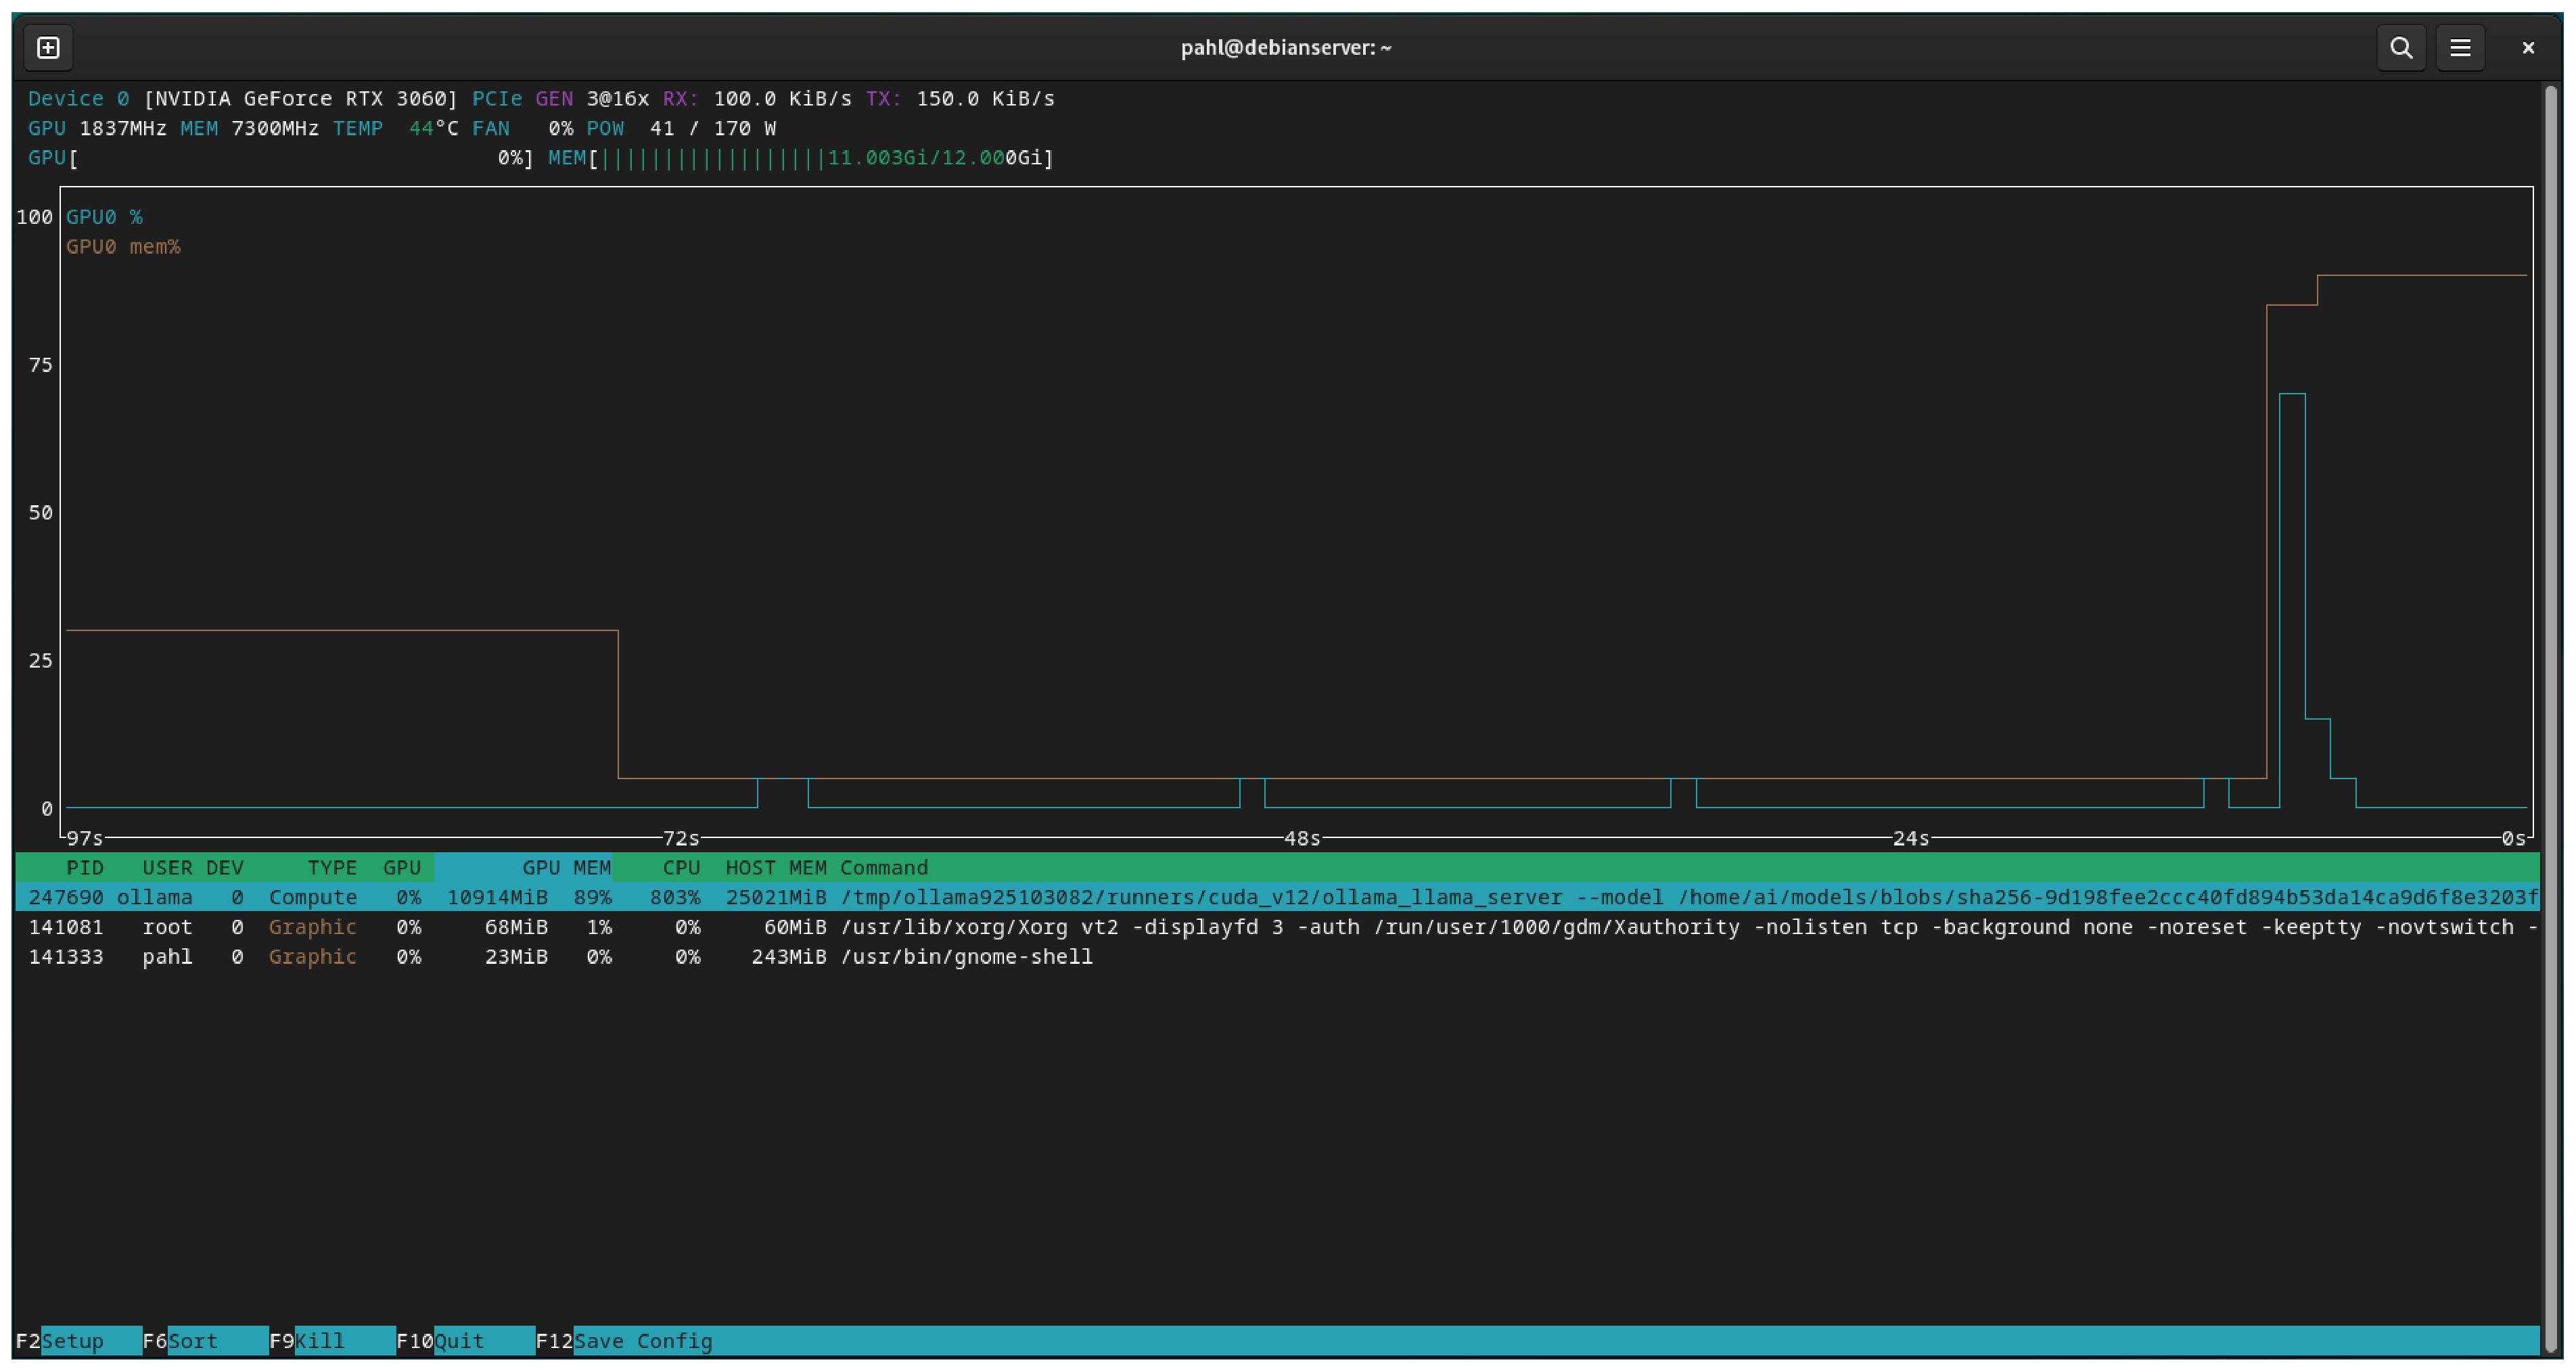
\includegraphics[width=0.8\textwidth]{content/chapter_lessons_learned/images/nvtop_model_change.eps}
	\centering
	\caption{Auslastung des VRAMs während eines Modellwechsels}
	\label{img:bash_nvtop_model_change}
\end{figure}

Die Abbildung \ref{img:bash_nvtop_model_change} zeigt den Modellwechsel vom \textit{Llama3.2} zum \textit{Codellama:70b} Modell. In der Abbildung werden die Grafikkartenparameter mit dem Tool \texttt{nvtop} ausgelesen und angezeigt. Während die Auslastung des VRAMs beim \textit{Llama3.2:3b} 3,64 GB beträgt, sind es beim \textit{Codellama:70b} mehr als 11 GB. Das \textit{Llama3.2:3b} hat eine tatsächliche Größe von 2 GB, während das \textit{Codellama:70b} eine tatsächliche Größe von 25 GB hat. Im linken Teil der Abbildung ist das geladene \textit{Llama3.2:3b} Modell zusehen, gefolgt von einem Leerlauf des Speichers zur Vorbereitung auf das neu zu ladende \textit{Codellama:70b} Modell. Die Speicherauslastung dieses Modells ist auf der rechten Seite der Abbildung \ref{img:bash_nvtop_model_change} zu erkennen. Ebenfalls wurde eine erhöhte Auslastung der CPUs beobachtet. Während die Auslastung bei der Verwendung des \textit{LLama3.2} Modells einen \texttt{Load average} von 0.12 hervorrief
%, was die Abbildung \ref{img:bash_htop_llama32} zeigt
, ist der Wert bei Ausführung des \textit{Codellama} Modells bei 7.53 und mehr gestiegen.
%, dies ist in Abbildung \ref{img:bash_htop_codellama} zu sehen.
Das Problem konnte nicht abschließend aufgeklärt werden.\vspace{0.2cm}

%\begin{figure}[!ht]
%	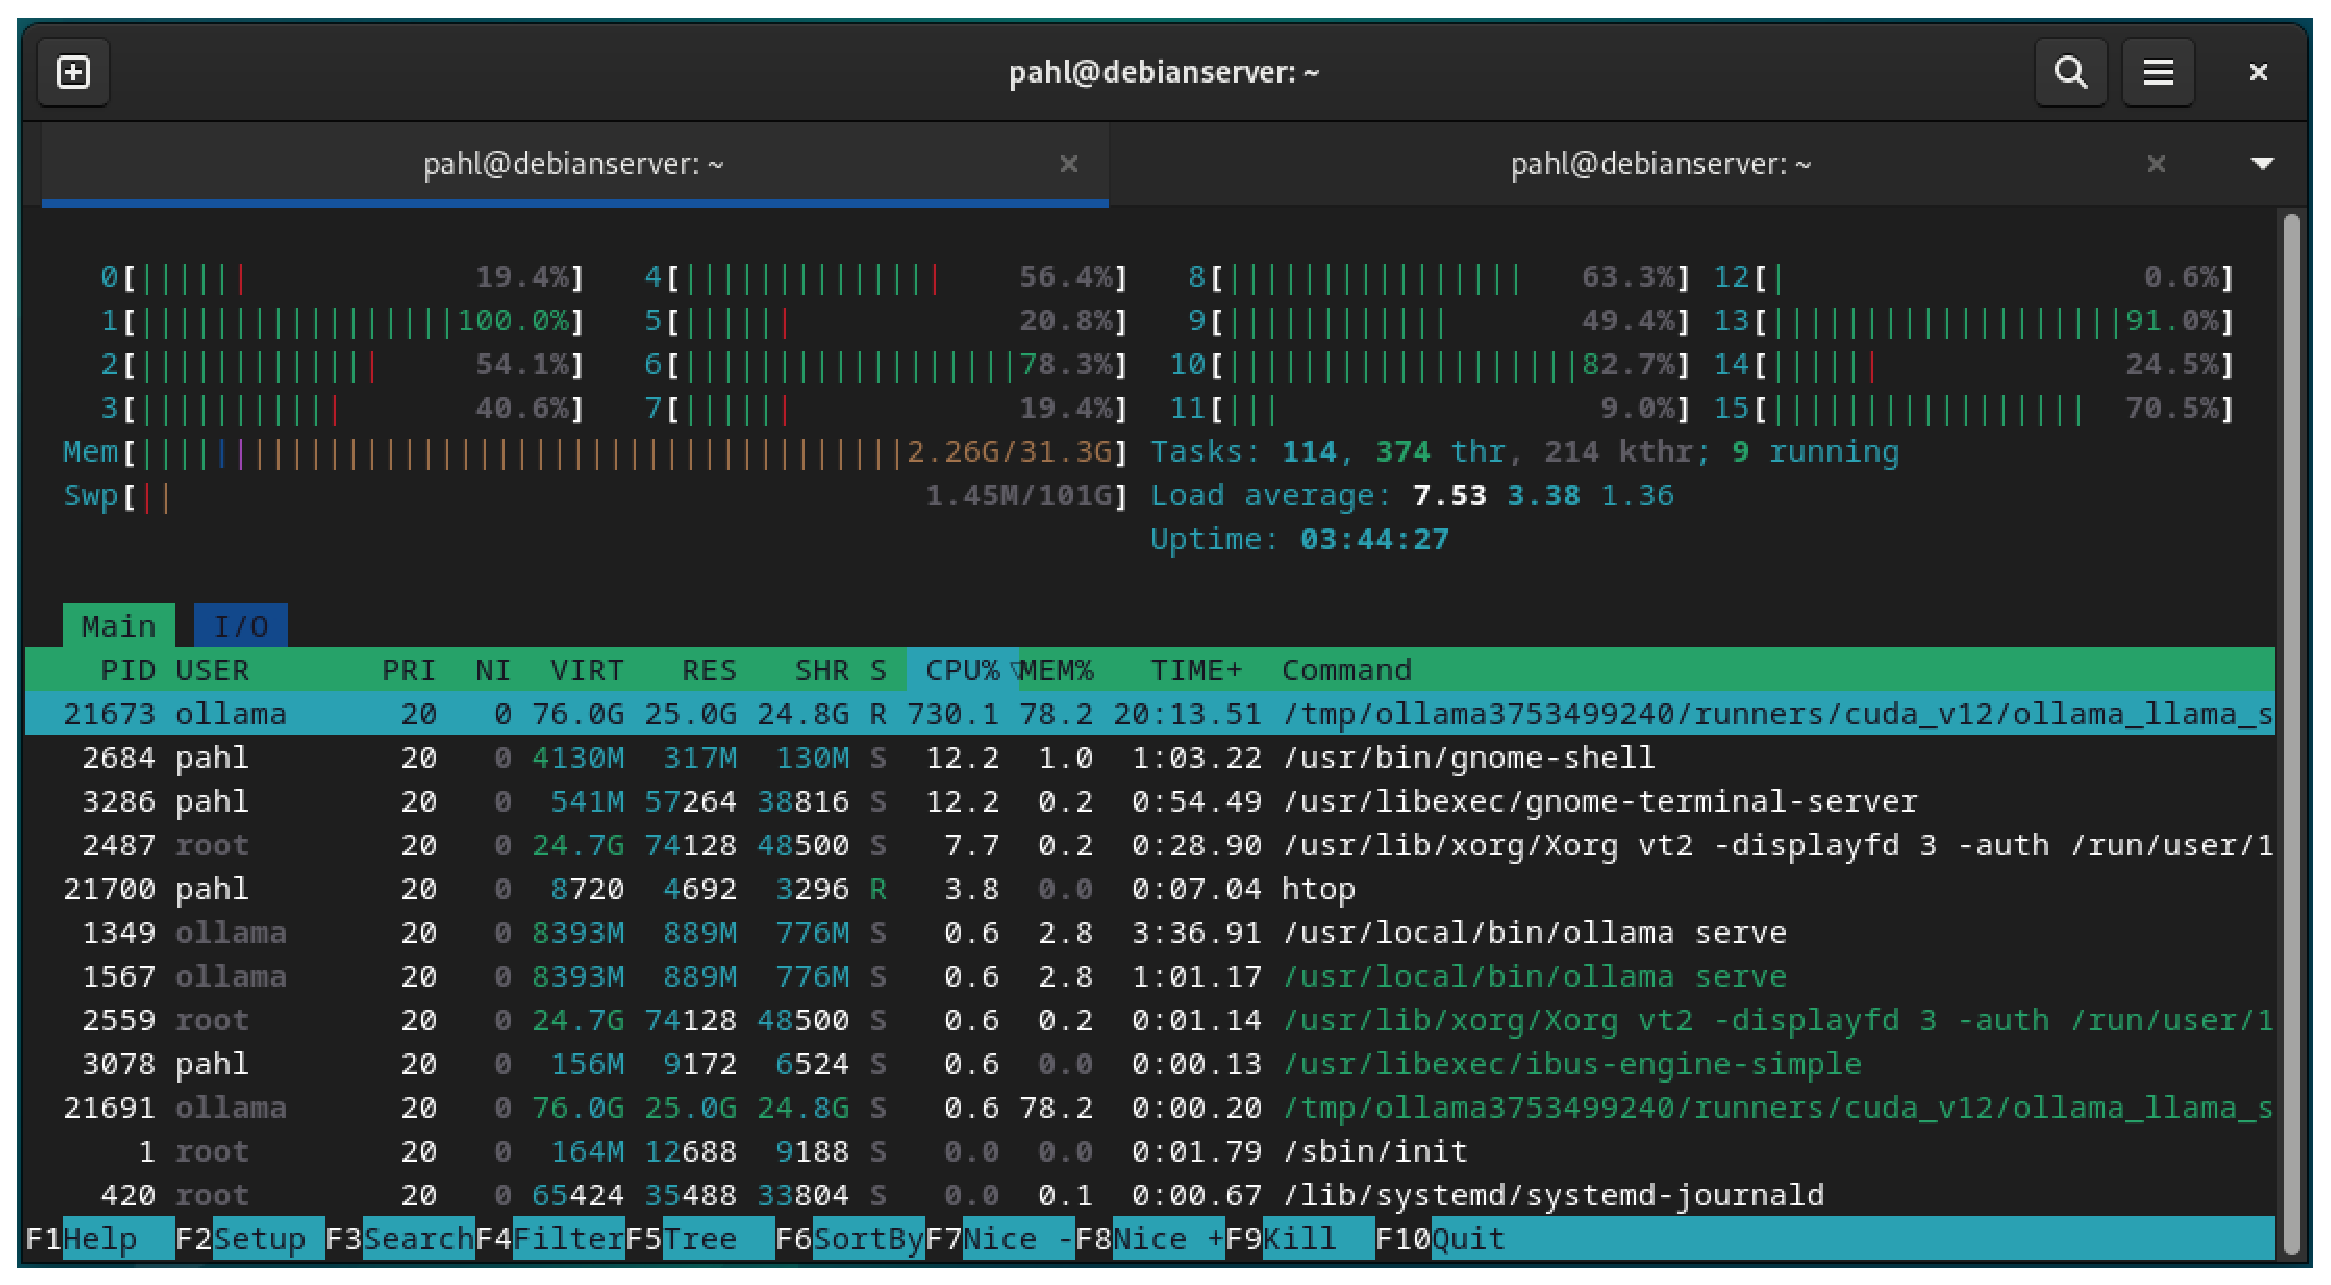
\includegraphics[width=0.8\textwidth]{content/chapter_lessons_learned/images/htop_ollama_working_codellama.eps}
%	\centering
%	\caption{Auslastung CPU bei der Codellama Ausführung}
%	\label{img:bash_htop_codellama}
%\end{figure}

%\begin{figure}[!ht]
%	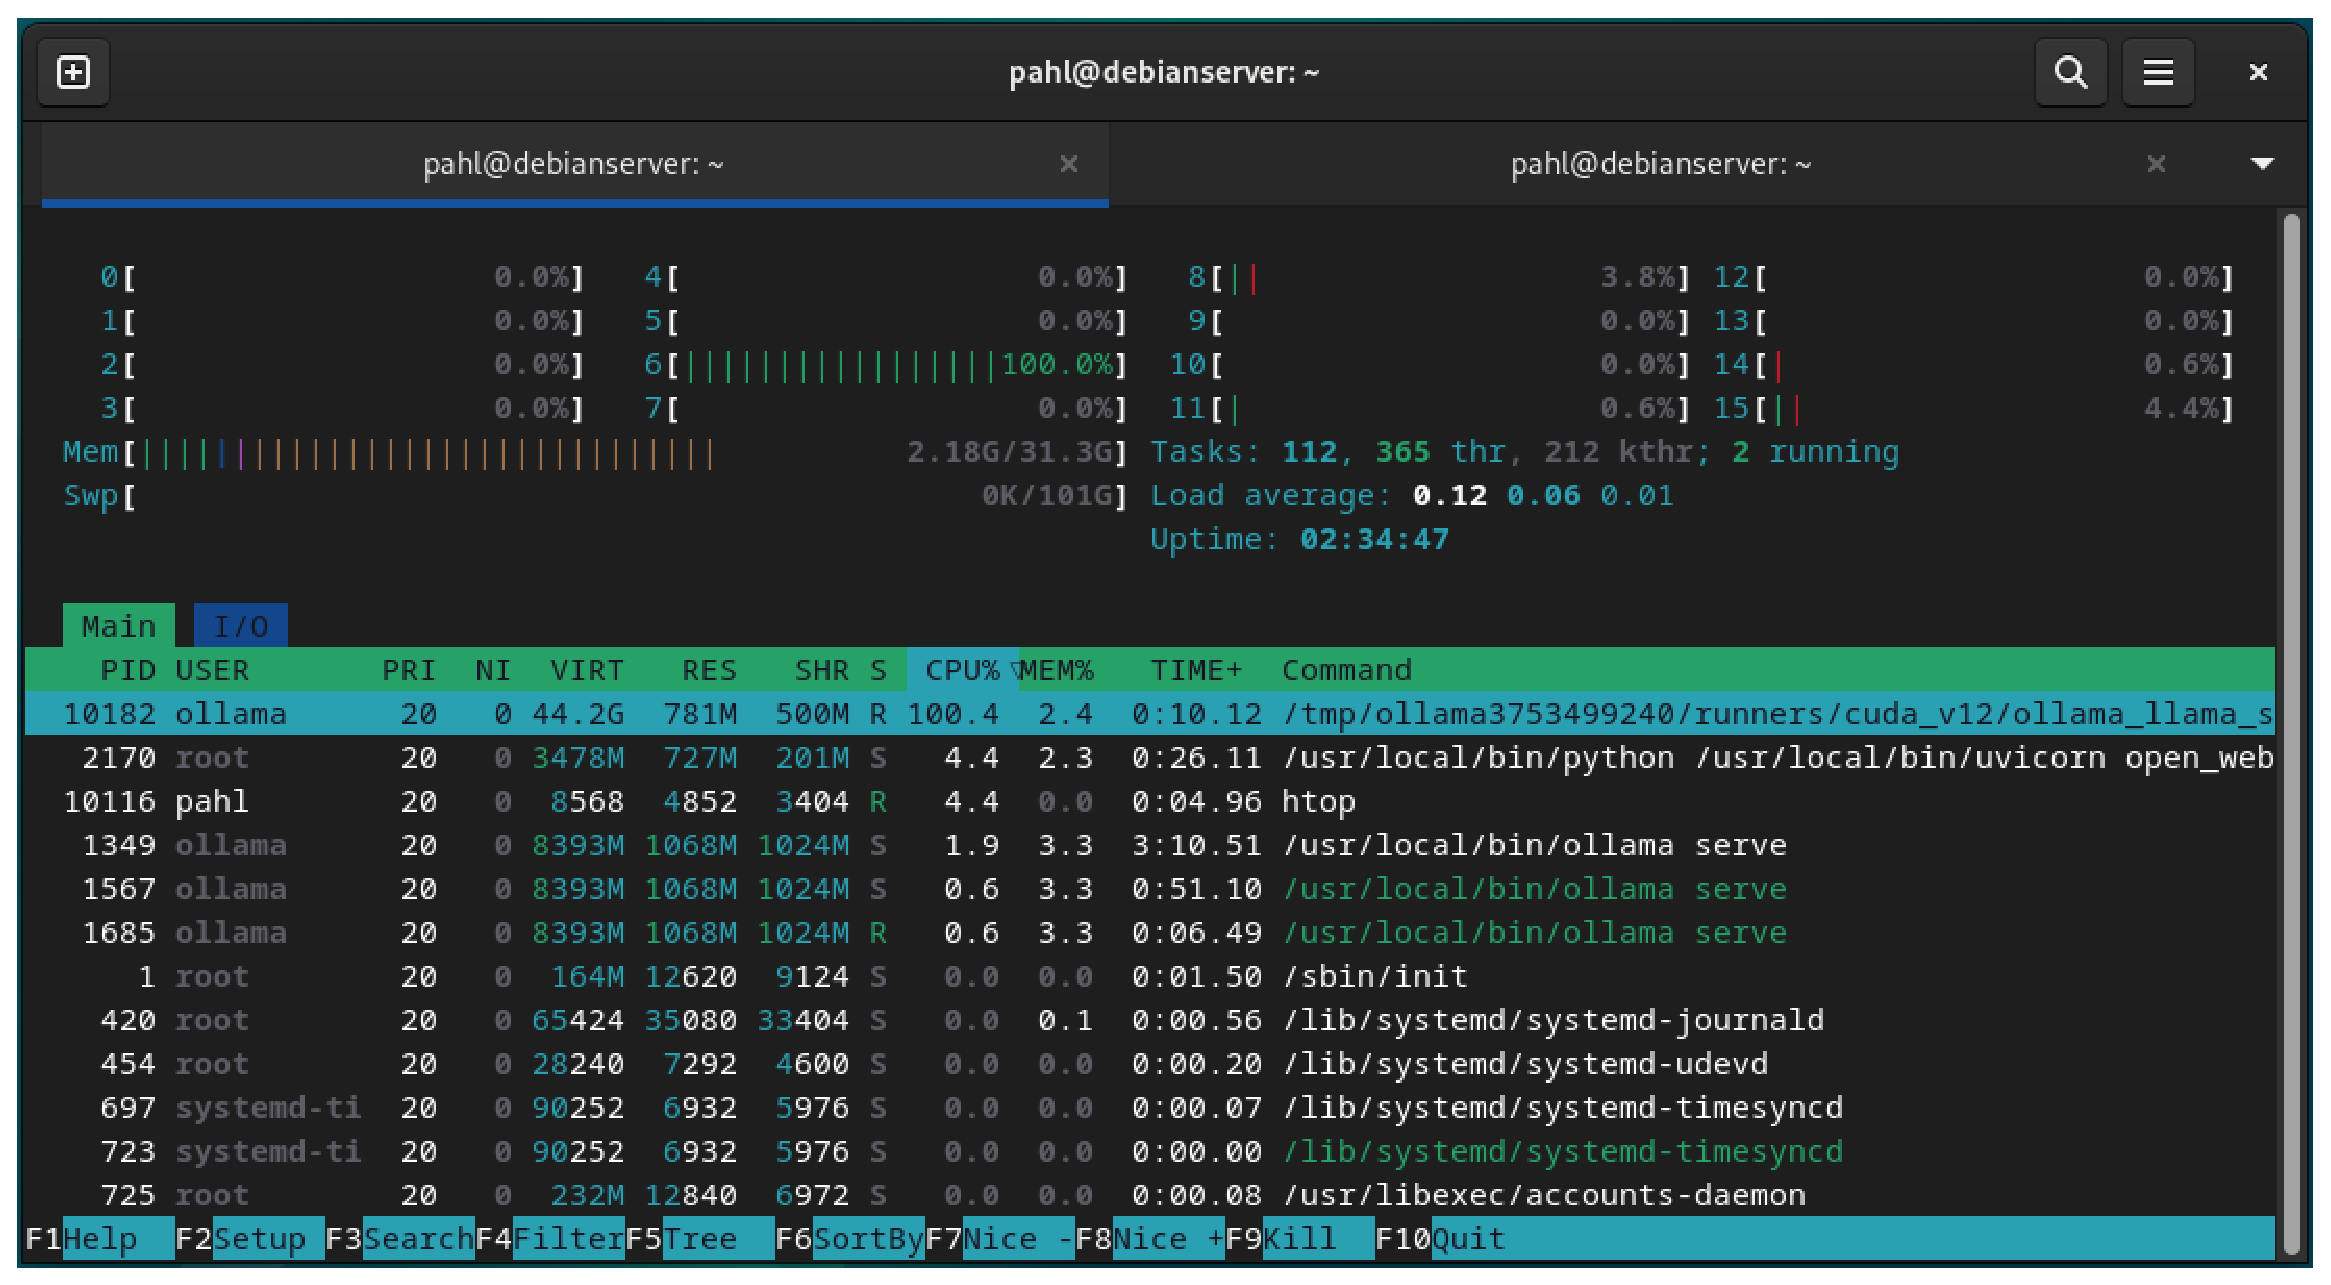
\includegraphics[width=0.8\textwidth]{content/chapter_lessons_learned/images/htop_ollama_working_llama32.eps}
%	\centering
%	\caption{Auslastung CPU bei der Llama 3.2 Ausführung}
%	\label{img:bash_htop_llama32}
%\end{figure}
